    \begin{comment}
    In order to describe the input and output combinations that would indicate a cell-aware fault occurred, we created something called a user defined fault model (UDFM). The generation of the UDFM itself was simple, the most difficult task came about when selecting possible input-output combinations that would indicate a cell-aware fault. We choose to select these combinations based on the key fact that cell-aware type faults are resistant to stuck-at ATPG. We took the standard cell library for which we were to generate the UDFM, and then created small verilog modules to describe each of the standard cells, and then performed stuck-at ATPG on these verilog modules. We then examined the pattern files that were generated and selected input combinations that would conflict with the truth table of the standard cell, and would also not be tested for by stuck at ATPG, and inserted them into the UDFM. 


    Targeting all of the possible cell-aware faults is costly, and impossible in most cases. There are a specific sub-class of cell aware faults that will affect the devices output or function during normal usage. The point of our study was to find an effective manor in which this sub-class can be specifically targeted by an ATPG tool. In short, when resources are limited we may only want to focus on faults that are especially likely to cause field errors, or functional faults. 



    To try and discover a methodology whereby the prediction of functional faults becomes a systematic process we had previously extracted circuit goodstate patterns. The premise was that by extracting these goodstates we have a list of possible states that the circuit can be in during functional usage. The goodstate patterns that were extracted included the contents of every state cell (i.e. flip flops and latches) for the circuit. Initially we used five ISCAS 1989 benchmark circuits, unfortunately it was very difficult to discover and provide functional inputs to the circuits. We instead generated a couple random input patterns for each of the five circuit that we were using. We then allowed the circuits to update for 40,000 clock cycles, and captured the contents of all the memory elements in the circuit after every clock cycle. Our thoughts were that no matter what the circuits function was, and no matter the inputs that it received, we could expect state values that would result during functional usage. 

    Because capturing these goodstates is expensive memory wise, we proceeded to think of ways that a similar analysis could be done during functional simulation. This would allow us to predict which faults would be most likely to cause errors during functional usage simultaneously, without having to store off goodstates and then reuse them. 

    We began this analysis by using ATPG on the faults described in the UDFM that we created earlier. This allowed us to see which state bits and inputs were mandatory for our cell-aware faults to be detected. Due to the nature of a test pattern propagating the fault to the output, it was evident that the test patterns generated would indeed see the faulty circuit values propagated to the outputs of the circuit. This means that if these patterns were to occur, then the fault would cause problems during the functional usage of the circuit. Because multiple patterns were generated for each of the faults that we described in the UDFM, it was possible to examine the the state bits, and input bits which didn't change for each input pattern, and to determine the bits that were set or reset in every pattern that detected the fault. These bits being either set or reset depending on the fault are a particular attribute of the circuit, and are called the mandatory conditions for fault detection or simply the mandatory conditions. 

    For example, imagine a small 4 input circuit with few gates. Imagine that we performed stuck-at ATPG on the circuit and in order to detect one of the stuck-at-0 faults the following 3 input patterns were given: 0010, 0110, 0111. In all three cases the first input bit is reset and the third is set, so the two mandatory conditions for detecting this stuck-at-0 fault are: input\_1 = 0, and input\_3 = 1. We performed this analysis for each of circuits, for each fault in the UDFM, and arrived at a long list of the mandatory conditions required for fault detection.  

    The next step was to monitor how many times the mandatory conditions were all met for each fault during functional simulation(running through each of the sets of goodstates we captured). This meant that we were able to gain a quantifiable value that was indicative of how many times a cell-aware fault would directly affect the output of the circuit. We should now be able to more effectively target only those specific faults that have a much greater bearing on the overall output of the circuit that is produced. 

    There are a few scenarios that are worthy of consideration before the results of this procedure are discussed. The first scenario arises when the total functionality of a circuit is known, and the goodstates that are captured are distributed equally among the state space of the device. In this case, using mandatory condition counts from functional simulation is probably a good indicator as to whether or not such faults should be targeted because the full functionality of the circuit is represented. On the other hand, the test engineers may have to contend with 3rd party IP, and can thus only know some of the total functionality of the circuit. This means that the goodstates they generate for functional simulation will be constrained to a much smaller portion of the entire space state, and in this case other considerations should be made when determining whether or not a fault should be tested for based on its functional application. 

    We are currently investigating a data encryption standard circuit DES56, and are performing a similar analysis to that which was performed on the ISCAS benchmark circuits. The major difference between the previous circuits and this one is that we understand the full functionality and have a working functional testbench for the encryption circuit, whereas it was very difficult to discern the purposes of the ISCAS circuits, and we had to resort to using random input vectors to generate their goodstates. In the analysis section we refer to the number of times that all the mandatory conditions were met for a particular fault during the functional simulation as that fault's ``mandatory count'' 
    \end{comment}

    \subsection{Cell-Aware Type UDFM Generation}
    In Section \ref{sec:caf} several types of faults were discussed, but in particular detail the cell-aware-type fault was introduced. 
    We also showed how to find a potential input vector that could be used to test for a cell-aware-type fault(by a nor-gate example). 
    The input vector, identified for cell-aware-type fault detection, was illustrated in Figure \ref{fig:caf}.
    Note that this represented only a single gate, and not a gate within a circuit. 
    The two circuits on which this analysis was performed are an ISCAS 89' benchmark circuit (s9234) and a DES56 encryption/decryption circuit from opencores.org.
    Each of them were synthesized using a different standard cell-library.
    These libraries included many different types of cells such as And-Or-Inverts, Half-Adders, and Three-Input NORs. 
    It became our task to develop a standard way of finding which patterns could be used to detect the cell-aware-type faults. 
    We did this in a very similar manner to the example in Section \ref{sec:caf}. 
    To automate the process, we used a standard stuck-at ATPG tool (Mentor Graphics Tessent)to generate the stuck-at test patterns so we didn't have to do it manually (as was shown in the example).
    We then cross-referenced each standard cells truth table, and determined what input pattern could be used to detect a fault within that cell. 
    Finally, to define a fault model that fit the input vectors we were generating, we used some built in functionality of the Tessent which allowed us to define our own fault model, a UDFM (User-Defined-Fault-Model).
    After generating a UDFM that properly represented several potential cell-aware-type fault input-output pairings,  we moved on to the next part of the experiment.

    \subsection{Mandatory Condition Extraction}
    To allow for the prediction of the importance of specific cell aware faults in a given circuit, we first had to extract an attribute of each fault individually. 
    As was shown before in section \ref{sec:caf}, certain input vectors are required to test for a given fault. 
    For the cell-aware fault in Figure \ref{fig:caf} only one such input vector was specified. 
    Granted, that circuit is only one gate and as such only one pattern could have potentially detected a cell-aware fault. 
    For larger more realistic circuits that consist of many gates, there are many different patterns that can detect the same fault.

    A certain feature of most ATPG tools called ``n-detect.'' 
    This approach allows for the user to specify a value of n. 
    The specified value is then used as a target for the tool to generate a set of patterns that detect each fault at least n times.
    Specifying a large value of n will return many patterns that detect the same fault in an output file format called a fault dictionary. 
    The fault dictionary is essentially just a cross-listing of patterns and the respective faults they detect. 
    We used a similar method to n-detect to allow for the generation of a fault dictionary, which we then examined to extract a general formula for patterns that could detect a given fault. 
    These formulas are henceforth referred to as the mandatory conditions for fault detection. 


    Imagine a circuit $C$ has a potential cell-aware fault $f$, six primary inputs, labeled: $p_{0}-p_{5}$, and 2 internal state elements (D-Flip-Flops, Latches, etc...), labeled $d_{0}-d_{1}$ from most significant to least significant.
    $C$ is large enough that four test patterns exist that can detect $f$. 
    Assume we set the n-value to some arbitrary number greater than four. 
    After running ATPG, using the UDFM generated above, the following patterns are described in the fault dictionary. 


    \begin{center}
    \begin{tabular}{| c | c | c |}
        \hline
        & Inputs & Flip-Flops\\
        \hline
        \hline
        Pattern 1 & \textcolor{red}{0}1011\textcolor{red}{1} & 0\textcolor{red}{0} \\
        \hline
        Pattern 2 & \textcolor{red}{0}0100\textcolor{red}{1} & 1\textcolor{red}{0} \\
        \hline
        Pattern 3 & \textcolor{red}{0}1111\textcolor{red}{1} & 0\textcolor{red}{0} \\
        \hline
        Pattern 4 & \textcolor{red}{0}0000\textcolor{red}{1} & 1\textcolor{red}{0} \\
        \hline
    \end{tabular}
    \end{center}

    Notice that the values in red do not change at all in any of the patterns, but that ever other bit changes. 
    There are three mandatory conditions, we denote the mandatory conditions of $f$ as $MC(f)$.
    We can now derive $MC(f)$ for this circuit, because we know all of the patterns that detect the fault. 
   
    In general, it is difficult to know how many patterns are capable of detecting a particular fault without exhaustive analysis. 
    Thus it is important that the value of n be selected be appropriately large to help increase the probabiliity that the identified conditions are truly mandatory. 

    \begin{center}
    \begin{Equation}
        $MC(f) = \overline{p_{0}}p_{5}\overline{d_{1}}$
    \end{Equation}
    \end{center}

    The next part of the setup is to count how many times these mandatory conditions are met during functional usage.
    However, we must first discuss how we performed functional simulation. 


    \subsection{Circuit Goodstate Extraction & Functional Simulation}

    For s9234, we did not know the original function of the circuit. 
    We intentionally allowed its intended function to remain obscured so we would only test for a certain small part of the overall state space. 
    This experiment is representative of rating the importance of cell-aware faults for a circuit whose function is unknown, or only one function of a group of many is known.
    This was to emulate a company using an obfuscated circuit of which they only know one intended use.
    We first inserted a scan chain into the circuit in order to allow for the extraction of state bits. 
    We then generated 40,000 random inputs, and extracted the total complement of state bits after each clock cycle. 
    We stored these as the first set of 40,000 goodstates, and then generated another set. 
    Finally we created a test bench which allowed the functional simulation of s9234, using the goodstates.


    For DES56 however, the intended purpose was known. 
    We also had a functional test bench for this circuit already which was used in previous research.
    We used the DES56 circuit to encrypt and decrypt the plain text ASCII version of this paper \cite{1299219}. 
    This qualifies as functional simulation of the circuit because it is realizing the intended purpose of both encryption and decryption. 
    We covered a much higher percentage of the state space during this functional simulation. 
    This was intended to emulate the testing of a circuit whose functionality is known in its entirety. 


    Lastly, we detected the number of times that a faults mandatory conditions were met during functional simulation.
    This was the key attribute that we intended to use for fault importance predictions. 
    We henceforth refer to this value as the ``mandatory count'' for a particular fault.
    This is discussed in the next subsection.
    

    \subsection{Mandatory Counts during Functional Simulation}
    As we have seen, the mandatory conditions for a given fault can be represented as a boolean function of the fault. 
    In the example above we determined that $MC(f) = \overline{p_{0}}p_{5}\overline{d_{1}}$. 
    The result that these mandatory conditions can be represented as a boolean function is essential. 
    By representing them as a boolean function we can add a few simple logic gates with an output signal that feeds a counter. 
    We created a script to read the mandatory conditions file that was created by parsing the fault dictionary. 
    This script output a testbench to allow for functional simulation of the circuit, but it added a few of these extra logic gates that allowed us to keep a count of how many times the mandatory conditions for each fault were met during functional simulation. 
    The logic gate that would be added to the circuits test bench in order to examine whether the mandatory conditions for the fault detailed above is given in Figure \ref{fig:mandgate}

\begin{figure}[h!]
\centering
\caption{Mandatory Condition Detector for fault f\label{fig:mandgate}}
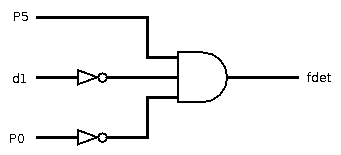
\includegraphics[scale=0.5]{Figures/mand.png}
\end{figure} 

    Because the mandatory conditions were generated based on test patterns that were engineered to propagate the fault to the outputs of the circuit, if they are met during functional simulation, then a device with this fault will output an erroneous value during its use.  
    We can use the mandatory counts for each fault to rank them in terms of their importance.
    They can then be sorted by the probability that they will cause problems during the functional use of the device. 
    In order to determine if the mandatory counts were a good indication of whether or not the fault would be detected during functional use, the last part of the experiment consisted of the use of a fault simulator to determine whether or not a fault would be detected during the same ``goodstates''. 
    We could then set a prediction criteria in terms of the mandatory counts for a particular circuit and construct a confusion matrix and calculate the corresponding statistics to determine how well these mandatory counts predicted whether or not a fault was truly functional (would be detected during fault simulation). 
    